\makesubsectionpage{Neuronale Netze}

\makesubsectionpage{Einlagiges Perzeptron}


\begin{frame}{Neuronale Netze: Einführung}
\begin{columns}
\column{0.60\textwidth}
\centering
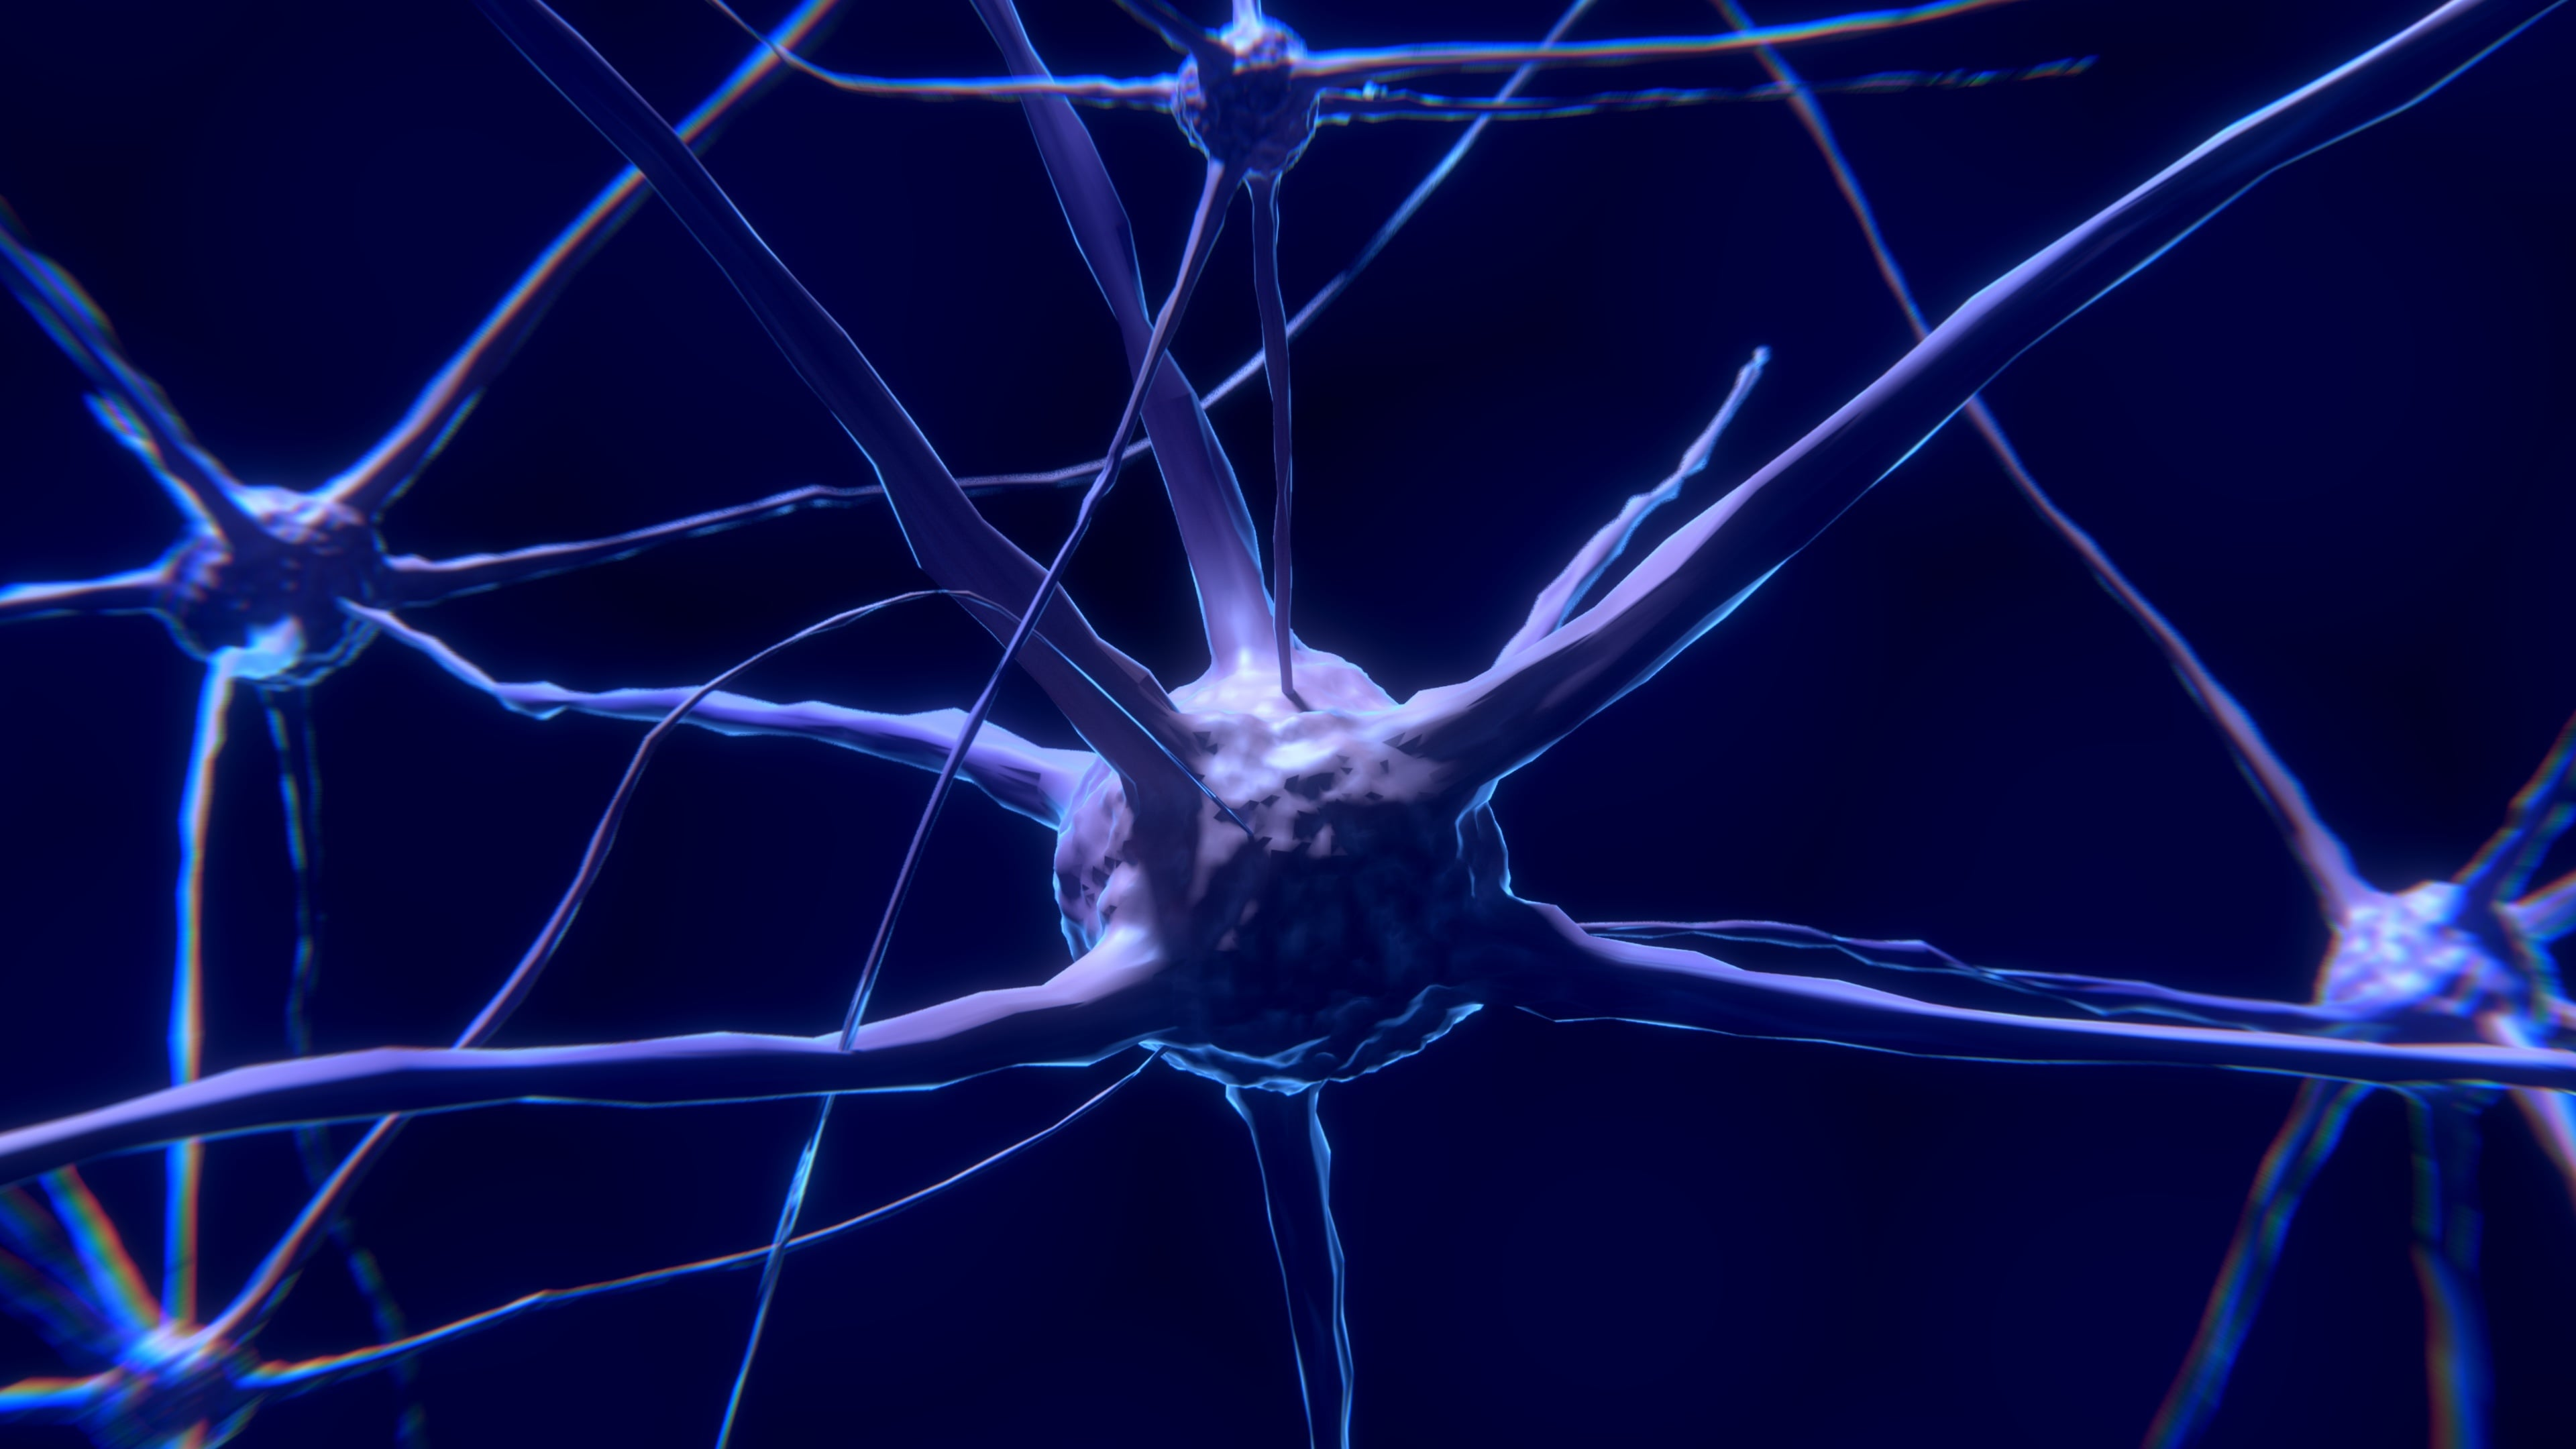
\includegraphics[width=\linewidth]{figures/neuronen.jpg}
\footnotesize Skizze vernetzter Neuronen

\column{0.35\textwidth}
\footnotesize
\begin{itemize}
  \item \textbf{Neuronale Netze} sind außerhalb der Fachwelt die
        bekanntesten Lernverfahren.
  \item Lange wurden sie kaum verwendet wegen ihrer starken Tendenz zur
        \textbf{Überanpassung}.
  \item Neuere Entwicklungen und aktuelle \textbf{Hardware} erlauben heute
        sehr komplexe, leistungsfähige Netze.
  \item Vorbild ist das \textbf{menschliche Gehirn} aus vernetzten
        \textbf{Neuronen}.
\end{itemize}
\end{columns}
\end{frame}


\begin{frame}{Neuronale Netze: Ursprung}
\begin{columns}
\column{0.60\textwidth}
\begin{itemize}
  \item Die Anfänge liegen bei \textbf{McCulloch und Pitts} in den 1940er
        Jahren.
  \item Ziel: einfaches \textbf{mathematisches Modell} für das
        Verhalten der Neuronen im Gehirn.
  \item In Medien werden Netze oft mit einem \textbf{künstlichen Gehirn} gleichgesetzt --
        das ist irreführend.
  \item Das Gehirn ist als Ganzes \textbf{nicht verstanden}; Netze lassen
        sich daher nicht über das Gehirn erklären.
  \item Hilfreicher ist der Blick auf die \textbf{Verkettung von
        Funktionen}.
\end{itemize}

\column{0.35\textwidth}
\centering
\resizebox{\linewidth}{!}{%
\begin{tikzpicture}[>=Stealth,
  neuron/.style={circle, draw=PrimaryColor, very thick,
                 minimum size=14pt, inner sep=0pt},
  input/.style={circle, fill=SecondaryColor, draw=SecondaryTitle,
                very thick, minimum size=14pt, inner sep=0pt},
  output/.style={circle, fill=AccentColor, draw=AccentTitle,
                 very thick, minimum size=14pt, inner sep=0pt}
]
% Input-Schicht
\node[input] (i1) at (0,2.4) {};
\node[input] (i2) at (0,1.2) {};
\node[input] (i3) at (0,0) {};
% Hidden-Schicht
\node[neuron] (h1) at (2,3.0) {};
\node[neuron] (h2) at (2,1.8) {};
\node[neuron] (h3) at (2,0.6) {};
\node[neuron] (h4) at (2,-0.6) {};
% Output-Schicht
\node[output] (o1) at (4,1.8) {};
\node[output] (o2) at (4,0.6) {};
% Kanten Input -> Hidden
\foreach \i in {1,2,3}
  \foreach \h in {1,2,3,4}
    \draw[->, gray] (i\i) -- (h\h);
% Kanten Hidden -> Output
\foreach \h in {1,2,3,4}
  \foreach \o in {1,2}
    \draw[->, gray] (h\h) -- (o\o);
% Beschriftung
\node[font=\scriptsize] at (0,-1.0) {Eingabe};
\node[font=\scriptsize] at (2,-1.4) {verdeckte Schicht};
\node[font=\scriptsize] at (4,-1.0) {Ausgabe};
\end{tikzpicture}}


\end{columns}
\source{\cite{Frochte2020}}
\end{frame}

\begin{frame}{Einlagiges Perzeptron: Das künstliche Neuron}
\begin{columns}
\column{0.47\textwidth}
\centering
\resizebox{\linewidth}{!}{%
\begin{tikzpicture}[>=Stealth,
  input/.style={circle, fill=SecondaryColor, draw=SecondaryTitle,
                very thick, minimum size=10pt, inner sep=0pt},
  sum/.style={circle, draw=PrimaryColor, very thick, minimum size=20pt},
  act/.style={rectangle, draw=PrimaryColor, very thick, minimum size=18pt},
  ausgabe/.style={circle, fill=AccentColor, draw=AccentTitle,
                  very thick, minimum size=10pt, inner sep=0pt}
]
% Inputs
\node[input] (x0) at (0,3.0) {};
\node[input] (x1) at (0,2.0) {};
\node[input] (x2) at (0,1.0) {};
\node[font=\scriptsize] at (0,0.2) {$\vdots$};
\node[input] (xn) at (0,-0.6) {};
\node[font=\scriptsize, left] at (-0.2,3.0) {$x_0$};
\node[font=\scriptsize, left] at (-0.2,2.0) {$x_1$};
\node[font=\scriptsize, left] at (-0.2,1.0) {$x_2$};
\node[font=\scriptsize, left] at (-0.2,-0.6) {$x_n$};
% Summation
\node[sum] (h) at (2.6,1.2) {$\sum$};
% Aktivierung
\node[act] (g) at (4.2,1.2) {$g$};
% Output
\node[ausgabe] (y) at (5.6,1.2) {};
\node[font=\scriptsize, right] at (5.8,1.2) {$y$};
% Kanten mit Gewichten
\draw[->] (x0) -- (h) node[midway, above, font=\scriptsize] {$w_0$};
\draw[->] (x1) -- (h) node[midway, above, font=\scriptsize] {$w_1$};
\draw[->] (x2) -- (h) node[midway, below, font=\scriptsize] {$w_2$};
\draw[->] (xn) -- (h) node[midway, below, font=\scriptsize] {$w_n$};
\draw[->] (h) -- (g) node[midway, above, font=\scriptsize] {$h$};
\draw[->] (g) -- (y);
\end{tikzpicture}}

\column{0.48\textwidth}
\begin{itemize}
  \item Elementarer Baustein ist das \textbf{künstliche Neuron}.
  \item Links stehen die Einträge $x_0, x_1, \dots, x_n$ des
        \textbf{Merkmalsvektors} $\mathbf{x}$.
  \item Sie werden mit \textbf{Gewichten} $w_i \in \mathbb{R}$ multipliziert
        und aufsummiert.
  \item Das Ergebnis $h$ geht in die \textbf{Aktivierungsfunktion} $g$, die
        die Ausgabe $y$ liefert.
\end{itemize}
\end{columns}
\source{\cite{Frochte2020}}
\end{frame}

\begin{frame}{Einlagiges Perzeptron: Summation und Analogie}
\begin{columns}
\column{0.60\textwidth}
\begin{itemize}
  \item Die gewichtete Summe ergibt die Funktion
        $h: \mathbb{R}^n \to \mathbb{R}$:
        \[
          h(\mathbf{x}) = \sum_{i=0}^{n} w_i x_i
        \]
  \item $h(\mathbf{x})$ ist der Eingangswert der \textbf{Aktivierungs\-%
        funktion} $g$.
  \item \textbf{Biologische Analogie:} Eine Nervenzelle summiert die
        Anregungen anderer Zellen.
  \item Übersteigt die Summe ein \textbf{Schwellenpotential}, \textbf{feuert}
        die Zelle.
\end{itemize}

\column{0.35\textwidth}
\begin{blockC1}{Vereinfachung}
Das Modell ist stark vereinfacht -- es ist nur eine \textbf{Anlehnung} an
die echte Nervenzelle.
\end{blockC1}
\end{columns}
\source{\cite{Frochte2020}}
\end{frame}

\begin{frame}{Einlagiges Perzeptron: Schwellwertfunktion}
\begin{columns}
\column{0.47\textwidth}
\begin{itemize}
  \item Die mathematische Nachbildung \textbf{feuert} ab Überschreitung
        eines \textbf{Schwellenwertes} $\theta$.
  \item Sie springt dabei von $0$ auf $1$ (\textbf{Sprungfunktion}).
  \item Unterhalb von $\theta$ ist das Neuron \textbf{inaktiv}:
        \[
          y = g(h) =
          \begin{cases}
            1 & \text{für } h > \theta\\
            0 & \text{für } h \leq \theta
          \end{cases}
        \]
\end{itemize}

\column{0.48\textwidth}
\centering
\resizebox{\linewidth}{!}{%
\begin{tikzpicture}[>=Stealth]
% Achsen
\draw[->, thick] (-2.5,0) -- (2.8,0) node[right] {$h$};
\draw[->, thick] (0,-0.4) -- (0,2.2) node[above] {$g(h)$};
% Ticks
\draw (0.08,1.6) -- (-0.08,1.6) node[left, font=\footnotesize] {$1$};
\draw (0.8,0.08) -- (0.8,-0.08) node[below, font=\footnotesize] {$\theta$};
% Schwellwertfunktion mit Schwelle theta
\draw[PrimaryColor, line width=1.2pt] (-2.5,0) -- (0.8,0);
\draw[PrimaryColor, line width=1.2pt] (0.8,1.6) -- (2.8,1.6);
\draw[PrimaryColor, line width=1.2pt, dashed] (0.8,0) -- (0.8,1.6);
\fill[PrimaryColor] (0.8,1.6) circle (2.5pt);
\draw[PrimaryColor, fill=white, line width=1.2pt] (0.8,0) circle (2.5pt);
\end{tikzpicture}}
\end{columns}
\source{\cite{Frochte2020}}
\end{frame}

\begin{frame}{Einlagiges Perzeptron: Kompaktere Darstellung}
    \small
\begin{columns}
\column{0.60\textwidth}
\begin{itemize}
  \item Das Neuron lässt sich \textbf{mathematisch kompakt} darstellen.
  \item Jeder Eintrag $x_i$ wird mit dem Gewicht $w_i$ multipliziert und
        aufsummiert:
        \[
          h(\mathbf{x}) = \sum_{i=0}^{n} w_i x_i
        \]
  \item Fasst man Gewichte und Eingabe als \textbf{Vektoren}
        $\mathbf{w} = (w_0, \dots, w_n)^T$ und
        $\mathbf{x} = (x_0, \dots, x_n)^T$ auf, wird daraus ein
        \textbf{Skalarprodukt}:
        \[
          h(\mathbf{x}) = \mathbf{w}\cdot\mathbf{x}
        \]
  \item Die Ausgabe ist dann $y = g(h(\mathbf{x})) = g(\mathbf{w}\cdot\mathbf{x})$.
\end{itemize}

\column{0.35\textwidth}
\begin{blockC1}{\small Ziel}
Eine \textbf{knappe Notation}, die Gewichtung, Summation und Aktivierung in
einem Ausdruck zusammenfasst.
\end{blockC1}
\end{columns}
\source{\cite{Frochte2020}}
\end{frame}


\begin{frame}{Perzeptron: Schwellwert als Trenngerade}
\small
\begin{columns}
\column{0.47\textwidth}
\begin{itemize}
  \item Wir nehmen jetzt noch den den Schwellwert $\theta$ hinzu und stellen um:
        \[
          h(\mathbf{x}) - \theta = \mathbf{w}\cdot\mathbf{x} - \theta = 0
        \]
  \item Das ist eine \textbf{Hyperebenen-Gleichung}, wie wir sie von den
        \textbf{SVMs} kennen.
  \item $\theta$ verschiebt die Hyperebene aus dem \textbf{Ursprung}
        heraus.
  \item Im 2D-Fall ist die Hyperebene eine \textbf{Gerade}:
        \[
          w_0 x_0 + w_1 x_1 - \theta = 0
        \]
\end{itemize}

\column{0.48\textwidth}
\centering
\resizebox{\linewidth}{!}{%
\begin{tikzpicture}[>=Stealth]
% Achsen
\draw[->, thick] (-0.5,0) -- (4.5,0) node[right] {$x$};
\draw[->, thick] (0,-0.5) -- (0,4.5) node[above] {$y$};
% Trenngerade h - theta = 0
\draw[AlertTitle, line width=1.2pt] (-0.3,4.2) -- (4.2,0.3);
\node[AlertTitle, font=\footnotesize, anchor=south west]
  at (2.3,1.9) {$0 = h - \theta$};
% Bereiche beschriften
\node[font=\footnotesize, align=center] at (1.0,1.0)
  {$h - \theta < 0$\\$g(h) = 0$};
\node[font=\footnotesize, align=center] at (3.3,3.3)
  {$h - \theta > 0$\\$g(h) = 1$};
\end{tikzpicture}}
\end{columns}
\source{\cite{Frochte2020}}
\end{frame}

\begin{frame}{Perzeptron: Schema mit Bias-Neuron}
\footnotesize
\begin{columns}
\column{0.47\textwidth}
\begin{itemize}
  \item Die Trennebene ist ja beschrieben durch $w ⋅ x - 𝜃 = 0$.
  \item Das \textbf{Aktivierungspotenzial} $\theta$ ist dabei \textbf{konstant}. 
  \item Mit fixiertem $\theta$ könnte die Hyperebene nur ihre
        \textbf{Steigung} ändern, nicht ihre \textbf{Verschiebung}.
  \item Lösung: ein zusätzlicher, konstant $1$-wertiger Input, das
        \textbf{Bias-Neuron}.
  \item Ergebnis ist das \textbf{einlagige Perzeptron}.
  \item \textbf{Hinweis:} $y_2$ zeigt den allgemeinen \textbf{Mehr-Output}-Fall.
        Für zwei Klassen genügt \textbf{ein} Output-Neuron.
\end{itemize}

\column{0.48\textwidth}
\centering
\resizebox{\linewidth}{!}{%
\begin{tikzpicture}[>=Stealth,
  input/.style={circle, fill=SecondaryColor, draw=SecondaryTitle,
                very thick, minimum size=16pt, inner sep=0pt},
  bias/.style={circle, fill=AccentColor, draw=AccentTitle,
               very thick, minimum size=16pt, inner sep=0pt},
  outp/.style={circle, fill=PrimaryColor, draw=PrimaryTitle,
               very thick, minimum size=16pt, inner sep=0pt}
]
% Beschriftung Schichten
\node[font=\footnotesize\bfseries, align=center] at (0,4.6) {Input\\layer};
\node[font=\footnotesize\bfseries, align=center] at (4,4.6) {Output-\\Layer};
% Input-Neuronen
\node[input] (x1) at (0,3.6) {};
\node[input] (x2) at (0,2.0) {};
\node[bias]  (b)  at (0,0.4) {$1$};
\node[font=\footnotesize, left] at (-0.6,3.6) {$x_1$};
\node[font=\footnotesize, left] at (-0.6,2.0) {$x_2$};
\draw[->] (-0.5,3.6) -- (x1);
\draw[->] (-0.5,2.0) -- (x2);
% Output-Neuronen
\node[outp] (y1) at (4,3.0) {};
\node[outp] (y2) at (4,1.2) {};
\node[font=\footnotesize, right] at (4.6,3.0) {$y_1$};
\node[font=\footnotesize, right] at (4.6,1.2) {$y_2$};
\draw[->] (y1) -- (4.5,3.0);
\draw[->] (y2) -- (4.5,1.2);
% Kanten mit Gewichten
\draw[->] (x1) -- (y1) node[fill=white, inner sep=1pt, pos=0.22, font=\scriptsize] {$w_{1,1}$};
\draw[->] (x1) -- (y2) node[fill=white, inner sep=1pt, pos=0.22, font=\scriptsize] {$w_{2,1}$};
\draw[->] (x2) -- (y1) node[fill=white, inner sep=1pt, pos=0.28,  font=\scriptsize] {$w_{1,2}$};
\draw[->] (x2) -- (y2) node[fill=white, inner sep=1pt, pos=0.28,  font=\scriptsize] {$w_{2,2}$};
\draw[->] (b)  -- (y1) node[fill=white, inner sep=1pt, pos=0.22,  font=\scriptsize] {$w_{1,3}$};
\draw[->] (b)  -- (y2) node[fill=white, inner sep=1pt, pos=0.28,  font=\scriptsize] {$w_{2,3}$};
\end{tikzpicture}}
\end{columns}
\source{\cite{Frochte2020}}
\end{frame}

\begin{frame}{Perzeptron: Matrix-Vektor-Darstellung}
\footnotesize
\begin{columns}
\column{0.60\textwidth}
\begin{itemize}
  \item Die Gewichte werden so nummeriert, dass die Summation eine
        \textbf{Matrix-Vektor-Multiplikation} wird. Mit
        \[
          W = \begin{pmatrix*}[r]
            w_{1,1} & w_{1,2} & w_{1,3}\\
            w_{2,1} & w_{2,2} & w_{2,3}
          \end{pmatrix*}
        \]
        gilt $\mathbf{h} = W\cdot\mathbf{x}$ und
        $\mathbf{y} = g(\mathbf{h}(\mathbf{x}))$.
  \item $g$ wird \textbf{komponentenweise} angewandt (Schwellwert-/%
        Heaviside-Funktion).
  \item Am Beispiel $y_1$ zeigt sich die Rolle des Bias-Neurons:
        \[
          h(\mathbf{x}) = w_{1,1}\cdot x_1 + w_{1,2}\cdot x_2 + w_{1,3}\cdot 1
        \]
  \item $w_{1,3}$ übernimmt die Rolle von $-\theta$.
\end{itemize}

\column{0.35\textwidth}
\begin{blockC1}{\footnotesize Ein Output-Neuron}
Beim Startbeispiel genügt \textbf{ein} Output. $W$ wird einzeilig und lässt
sich als \textbf{Zeilen-Vektor} schreiben:
\[
  \mathbf{w} = \begin{pmatrix} w_1 & w_2 & w_3 \end{pmatrix}
\]
\end{blockC1}
\end{columns}
\source{\cite{Frochte2020}}
\end{frame}

\begin{frame}{Perzeptron: Hebbsche Lernregel}
\begin{columns}
\column{0.60\textwidth}
\begin{itemize}
  \item Neuronale Netze werden trainiert, indem man die \textbf{Gewichte} $w_i$ anpasst.
  \item Grundlage ist der \textbf{Fehler} zwischen gewünschtem $\hat{y}$ und
        beobachtetem $y$:
        \[
          \text{error} = \hat{y} - y
        \]
  \item Ist $\hat{y} > y$, werden die Gewichte \textbf{vergrößert}, sonst
        \textbf{verkleinert}:
        \[
          \Delta w_j = \text{error}\cdot x_j, \qquad w_j = w_j + \Delta w_j
        \]
  \item Eine \textbf{Lernrate} $\eta \in\, ]0,1]$ \textbf{dämpft} die
        Änderung und sichert die Konvergenz.
\end{itemize}

\column{0.35\textwidth}
\begin{blockC1}{Grundidee}
Gewichte mit \textbf{großem Einfluss} werden stärker verändert als solche
mit kleinem Einfluss.
\end{blockC1}
\end{columns}
\source{\cite{Frochte2020}}
\end{frame}

\begin{frame}{Perzeptron: Algorithmus der Hebbschen Lernregel}
\footnotesize
\begin{columns}
\SetAlgoCaptionLayout{footnotesize}      
\column{0.60\textwidth}
\begin{algorithm}[H]
\SetAlgoLined
\KwIn{Beispielmenge $D = \{(X, Y)\}$}
\KwOut{Gewichtsvektor $\mathbf{w}$}
$\mathbf{w}$ mit Zufallszahlen in $[-0.5, 0.5]$ initialisieren\;
$t = 0$\;
\Repeat{$\lVert Y - \text{heaviside}(WX)\rVert < \varepsilon$ \textbf{oder} $t > t_{\max}$}{
  $t = t + 1$\;
  $(\hat{x}, \hat{y}) = \text{RandomSelect}(D)$\;
  $\text{error} = \hat{y} - \text{heaviside}(W \cdot \hat{x})$\;
  \For{$j = 0$ \KwTo $p$}{
    $\Delta w_j = \eta\cdot\text{error}\cdot\hat{x}_j$\;
    $w_j = w_j + \Delta w_j$\;
  }
}
\caption{Hebbsche Lernregel}
\end{algorithm}

\column{0.35\textwidth}
\begin{blockC1}{\footnotesize Ablauf}
\begin{itemize}
  \item Zufälliges Beispiel $(\hat{x}, \hat{y})$ wählen.
  \item \textbf{Fehler} bestimmen:
        $\text{error} = \hat{y} - \text{heaviside}(W \cdot \hat{x})$.
  \item Pro Gewicht die Änderung berechnen:
        $\Delta w_j = \eta\cdot\text{error}\cdot\hat{x}_j$.
  \item Gewicht anpassen: $w_j = w_j + \Delta w_j$.
  \item Wiederholen, bis der Fehler $< \varepsilon$ ist oder $t_{\max}$
        erreicht ist.
\end{itemize}
\end{blockC1}
\end{columns}
\source{\cite{Frochte2020}}
\end{frame}

\begin{frame}{Hebbsche Lernregel -- Eigenschaften}
\begin{columns}
\begin{column}{0.6\textwidth}
\begin{itemize}
    \item Der Lernalgorithmus verwendet \textbf{Zufallszahlen} $\Rightarrow$ seed beeinflußt Ergebnis.
    \item Er liefert eine \textbf{Trennebene}, aber \textbf{keine optimale} im geometrischen Sinn.
    \item Qualität der Lösung variiert.
    \item Weitere Verfeinerungen möglich und notwendig.
    \item Dennoch bemerkenswert: funktionierender Lernalgorithmus \textbf{seit 1947}.
\end{itemize}
\end{column}

\begin{column}{0.35\textwidth}
      \centering
      \scriptsize 
\includesvg[width=0.8\linewidth]{figures/perceptron_trenngerade_42.svg}
Trenngerade mit seed=42
\vspace{0.5em}

\includesvg[width=0.8\linewidth]{figures/perceptron_trenngerade_100.svg}
Trenngerade mit seed=100
\end{column}

\end{columns}
\source{Perceptron\_Hebb.ipynb}
\end{frame}

\makequizpage{\QUIZURL}{\QUIZQRCODE}{\QUIZIMAGE}
\makequestionspage{\FRAGENIMAGE}


\makesubsectionpage{Multilayer Perceptron}

\begin{frame}{Was kann ein einlagiges Perzeptron wirklich?}

\begin{columns}

\column{0.55\textwidth}
\footnotesize
\begin{itemize}
    \item Ein einlagiges Perzeptron trennt Klassen exakt, wenn die Daten \textbf{linear separierbar} sind.
    \item \textbf{OR}: $(0,0)$ liefert $0$, alle anderen $1$. Der Nullpunkt lässt sich mit \textbf{einer Geraden} abtrennen $\Rightarrow$ \textbf{lernbar}.
    \item \textbf{AND}: $(1,1)$ liefert $1$, alle anderen $0$. Der Einspunkt ist mit \textbf{einer Geraden} abtrennbar $\Rightarrow$ \textbf{lernbar}.
    \item \textbf{XOR}: $(0,1)$ und $(1,0)$ liefern $1$, $(0,0)$ und $(1,1)$ liefern $0$. Die beiden Klassen liegen \textbf{über Kreuz} $\Rightarrow$ \textbf{keine Gerade} trennt sie.
    \item XOR ist daher \textbf{nicht linear separierbar}. Wir brauchen \textbf{mehrschichtige} Netze.
    \item Das \textbf{XOR}-Problem ist eines der berühmtesten Probleme der KI. 
\end{itemize}

\column{0.40\textwidth}
\centering
\resizebox{\linewidth}{!}{%
\begin{tikzpicture}[line cap=round, line join=round]
    \def\Axis{3.20}
    \def\Pos{2.00}
    \def\Rad{5pt}

    \pgfmathsetmacro{\SepOR}{0.5*\Pos}
    \pgfmathsetmacro{\SepAND}{1.5*\Pos}

    \tikzset{
        axis/.style={->, draw=black, line width=0.5pt},
        helper/.style={draw=black!28, line width=0.4pt},
        sep/.style={draw=AlertColor, line width=1.2pt},
        one/.style={circle, minimum size=2*\Rad, inner sep=0pt, draw=PrimaryTitle, fill=PrimaryColor, line width=1.0pt},
        zero/.style={circle, minimum size=2*\Rad, inner sep=0pt, draw=AccentTitle, fill=AccentColor, line width=1.0pt},
        lab/.style={font=\scriptsize, text=black},
        title/.style={font=\normalsize\bfseries, text=SecondaryTitle}
    }

    % OR
    \begin{scope}[xshift=0cm, yshift=3.10cm]
        \draw[axis] (0,0) -- (\Axis,0) node[right, black] {$x_1$};
        \draw[axis] (0,0) -- (0,\Axis) node[above, black] {$x_2$};

        \draw[helper] (0,\Pos) -- (\Pos,\Pos) -- (\Pos,0);

        \node[lab, below left] at (0,0) {$0$};
        \node[lab] at (\Pos,-0.32) {$1$};
        \node[lab] at (-0.32,\Pos) {$1$};

        \node[zero] at (0,0) {};
        \node[one] at (\Pos,0) {};
        \node[one] at (0,\Pos) {};
        \node[one] at (\Pos,\Pos) {};

        \draw[sep] (-0.15,\SepOR+0.15) -- (\SepOR+0.15,-0.15);

        \node[title] at (1.00,-0.70) {OR};
    \end{scope}

    % AND
    \begin{scope}[xshift=4.35cm, yshift=3.10cm]
        \draw[axis] (0,0) -- (\Axis,0) node[right, black] {$x_1$};
        \draw[axis] (0,0) -- (0,\Axis) node[above, black] {$x_2$};

        \draw[helper] (0,\Pos) -- (\Pos,\Pos) -- (\Pos,0);

        \node[lab, below left] at (0,0) {$0$};
        \node[lab] at (\Pos,-0.32) {$1$};
        \node[lab] at (-0.32,\Pos) {$1$};

        \node[zero] at (0,0) {};
        \node[zero] at (\Pos,0) {};
        \node[zero] at (0,\Pos) {};
        \node[one] at (\Pos,\Pos) {};

        \draw[sep] (-0.15,\SepAND+0.15) -- (\SepAND+0.15,-0.15);

        \node[title] at (1.00,-0.70) {AND};
    \end{scope}

    % XOR
    \begin{scope}[xshift=2.18cm, yshift=-1.5cm]
        \draw[axis] (0,0) -- (\Axis,0) node[right, black] {$x_1$};
        \draw[axis] (0,0) -- (0,\Axis) node[above, black] {$x_2$};

        \draw[helper] (0,\Pos) -- (\Pos,\Pos) -- (\Pos,0);

        \node[lab, below left] at (0,0) {$0$};
        \node[lab] at (\Pos,-0.32) {$1$};
        \node[lab] at (-0.32,\Pos) {$1$};

        \node[zero] at (0,0) {};
        \node[one] at (\Pos,0) {};
        \node[one] at (0,\Pos) {};
        \node[zero] at (\Pos,\Pos) {};

        \node[title] at (1.00,-0.70) {XOR};
    \end{scope}
\end{tikzpicture}}

\end{columns}

\source{\cite{Frochte2020}}
\end{frame}


\begin{frame}{Einlagiges Perzeptron für OR}
\footnotesize
\begin{columns}

\column{0.47\textwidth}
\begin{itemize}
    \item Das \textbf{Perzeptron} kann \textbf{analytisch} bestimmt werden.
    \item Für die Eingänge gelten die Gewichte
    \[
        w_1 = 1,\qquad w_2 = 1.
    \]
    \item Das \textbf{Bias-Gewicht} lautet
    \[
        w_3 = -0.5.
    \]
    \item Im \textbf{Output-Neuron} wird die \textbf{Heaviside-Funktion} verwendet:
    \[
        y = H(x_1 + x_2 - 0.5).
    \]
\end{itemize}

\column{0.48\textwidth}
\centering
\resizebox{\linewidth}{!}{%
\begin{tikzpicture}[>=Stealth,
  input/.style={circle, fill=SecondaryColor, draw=SecondaryTitle,
                very thick, minimum size=16pt, inner sep=0pt},
  bias/.style={circle, fill=AccentColor, draw=AccentTitle,
               very thick, minimum size=16pt, inner sep=0pt},
  outp/.style={circle, fill=PrimaryColor, draw=PrimaryTitle,
               very thick, minimum size=16pt, inner sep=0pt}
]
\node[font=\footnotesize\bfseries] at (2,4.6) {OR-Funktion};

\node[font=\footnotesize\bfseries, align=center] at (0,4.0) {Input\\layer};
\node[font=\footnotesize\bfseries, align=center] at (4,4.0) {Output-\\Layer};

\node[input] (x1) at (0,3.0) {};
\node[input] (x2) at (0,1.6) {};
\node[bias]  (b)  at (0,0.2) {$1$};

\node[font=\footnotesize, left] at (-0.6,3.0) {$x_1$};
\node[font=\footnotesize, left] at (-0.6,1.6) {$x_2$};

\draw[->] (-0.45,3.0) -- (x1);
\draw[->] (-0.45,1.6) -- (x2);

\node[outp] (y) at (4,1.6) {};
\node[font=\footnotesize, right] at (4.6,1.6) {$y$};
\draw[->] (y) -- (4.5,1.6);

\draw[->] (x1) -- (y) node[fill=white, inner sep=1pt, pos=0.48, font=\scriptsize] {$1$};
\draw[->] (x2) -- (y) node[fill=white, inner sep=1pt, pos=0.50, font=\scriptsize] {$1$};
\draw[->] (b)  -- (y) node[fill=white, inner sep=1pt, pos=0.48, font=\scriptsize] {$-0.5$};
\end{tikzpicture}%
}

\end{columns}

\source{\cite{Frochte2020}}
\end{frame}

\begin{frame}{Einlagiges Perzeptron für AND}
\footnotesize
\begin{columns}

\column{0.47\textwidth}
\begin{itemize}
    \item Auch dieses \textbf{Perzeptron} lässt sich \textbf{analytisch} angeben.
    \item Für die Eingänge gelten wieder die Gewichte
    \[
        w_1 = 1,\qquad w_2 = 1.
    \]
    \item Das \textbf{Bias-Gewicht} ist nun
    \[
        w_3 = -1.5.
    \]
    \item Im \textbf{Output-Neuron} wird die \textbf{Heaviside-Funktion} verwendet:
    \[
        y = H(x_1 + x_2 - 1.5).
    \]
\end{itemize}

\column{0.48\textwidth}
\centering
\resizebox{\linewidth}{!}{%
\begin{tikzpicture}[>=Stealth,
  input/.style={circle, fill=SecondaryColor, draw=SecondaryTitle,
                very thick, minimum size=16pt, inner sep=0pt},
  bias/.style={circle, fill=AccentColor, draw=AccentTitle,
               very thick, minimum size=16pt, inner sep=0pt},
  outp/.style={circle, fill=PrimaryColor, draw=PrimaryTitle,
               very thick, minimum size=16pt, inner sep=0pt}
]
\node[font=\footnotesize\bfseries] at (2,4.6) {AND-Funktion};

\node[font=\footnotesize\bfseries, align=center] at (0,4.0) {Input\\Layer};
\node[font=\footnotesize\bfseries, align=center] at (4,4.0) {Output\\Layer};

\node[input] (x1) at (0,3.0) {};
\node[input] (x2) at (0,1.6) {};
\node[bias]  (b)  at (0,0.2) {$1$};

\node[font=\footnotesize, left] at (-0.6,3.0) {$x_1$};
\node[font=\footnotesize, left] at (-0.6,1.6) {$x_2$};

\draw[->] (-0.45,3.0) -- (x1);
\draw[->] (-0.45,1.6) -- (x2);

\node[outp] (y) at (4,1.6) {};
\node[font=\footnotesize, right] at (4.6,1.6) {$y$};
\draw[->] (y) -- (4.5,1.6);

\draw[->] (x1) -- (y) node[fill=white, inner sep=1pt, pos=0.48, font=\scriptsize] {$1$};
\draw[->] (x2) -- (y) node[fill=white, inner sep=1pt, pos=0.50, font=\scriptsize] {$1$};
\draw[->] (b)  -- (y) node[fill=white, inner sep=1pt, pos=0.48, font=\scriptsize] {$-1.5$};
\end{tikzpicture}%
}

\end{columns}

\source{\cite{Frochte2020}}
\end{frame}

\begin{frame}{Mehrschichtige Netze: Motivation}
\begin{columns}
\column{0.55\textwidth}
\begin{itemize}
  \item Für \textbf{XOR} lassen sich keine passenden Gewichte $w$ finden.
  \item Lösung: mehrere Neuronen \textbf{neben-} und vor allem
        \textbf{hintereinander} verschalten.
  \item Solche Netze sind \textbf{weit komplexer} zu trainieren.
  \item Das Training nutzt \textbf{mathematische Optimierung} auf Basis von
        \textbf{Ableitungen}.
  \item Problem: die \textbf{Heaviside-Funktion} ist \textbf{nicht
        differenzierbar}.
\end{itemize}

\column{0.40\textwidth}
\begin{blockC1}{Konsequenz}
Wir brauchen \textbf{differenzierbare} Aktivierungsfunktionen als Ersatz für
die Heaviside-Funktion.
\end{blockC1}
\end{columns}
\source{\cite{Frochte2020}}
\end{frame}

\begin{frame}{Mehrschichtige Netze: Aktivierungsfunktionen}
\begin{columns}
\column{0.60\textwidth}
Zwei differenzierbare Alternativen zur Heaviside-Funktion:
\[
  \varphi = \text{sig}(ax) = \frac{1}{1 + \exp(-ax)}
\]
\[
  \phi = \tanh(ax) = \frac{e^{ax} - e^{-ax}}{e^{ax} + e^{-ax}}
\]

\begin{itemize}
  \item Wertebereich: \textbf{sig} zwischen $0$ und $1$, \textbf{tanh}
        zwischen $-1$ und $1$.
  \item Der Parameter $a$ steuert die \textbf{Steilheit}: je größer $a$,
        desto näher an der \textbf{Heaviside}-Funktion.
  \item Die Graphen zeigen den Fall $a = 5$.
\end{itemize}

\column{0.35\textwidth}
\centering
\resizebox{\linewidth}{!}{%
\begin{tikzpicture}[>=Stealth]
% ===== Sigmoid (y-Achse doppelt skaliert) =====
\begin{scope}[yshift=2.7cm]
\draw[->, thick] (-2.3,0) -- (2.3,0) node[right, font=\scriptsize] {$x$};
\draw[->, thick] (0,-0.2) -- (0,2.5) node[above, font=\scriptsize] {$y$};
\draw (0.05,2) -- (-0.05,2) node[left, font=\scriptsize] {$1$};
\draw (0.05,1) -- (-0.05,1) node[left, font=\scriptsize] {$0{,}5$};
\draw (2,0.05) -- (2,-0.05) node[below, font=\scriptsize] {$2$};
\draw (-2,0.05) -- (-2,-0.05) node[above, font=\scriptsize] {$-2$};
\draw[AccentColor, line width=1pt]
  (-2,0.0) -- (-1.5,0.001) -- (-1,0.013) -- (-0.7,0.059) --
  (-0.5,0.152) -- (-0.4,0.238) -- (-0.3,0.365) -- (-0.25,0.445) --
  (-0.2,0.538) -- (-0.15,0.642) -- (-0.1,0.755) -- (-0.05,0.876) --
  (0,1.0) -- (0.05,1.124) -- (0.1,1.245) -- (0.15,1.358) --
  (0.2,1.462) -- (0.25,1.555) -- (0.3,1.635) -- (0.4,1.762) --
  (0.5,1.848) -- (0.7,1.941) -- (1,1.987) -- (1.5,1.999) -- (2,2.0);
\node[AccentColor, font=\scriptsize] at (1,2.3) {$\text{sig}(5x)$};
\end{scope}

% ===== Tanh =====
\begin{scope}[yshift=-0.0cm]
\draw[->, thick] (-2.3,0) -- (2.3,0) node[right, font=\scriptsize] {$x$};
\draw[->, thick] (0,-1.3) -- (0,1.5) node[above, font=\scriptsize] {$y$};
\draw (0.05,1) -- (-0.05,1) node[left, font=\scriptsize] {$1$};
\draw (0.05,-1) -- (-0.05,-1) node[left, font=\scriptsize] {$-1$};
\draw (2,0.05) -- (2,-0.05) node[below, font=\scriptsize] {$2$};
\draw (-2,0.05) -- (-2,-0.05) node[below, font=\scriptsize] {$-2$};
\draw[SecondaryColor, line width=1pt]
  (-2,-1.0) -- (-1.5,-1.0) -- (-1,-1.0) -- (-0.7,-0.998) --
  (-0.5,-0.987) -- (-0.4,-0.964) -- (-0.3,-0.905) -- (-0.25,-0.848) --
  (-0.2,-0.762) -- (-0.15,-0.635) -- (-0.1,-0.462) -- (-0.05,-0.245) --
  (0,0.0) -- (0.05,0.245) -- (0.1,0.462) -- (0.15,0.635) --
  (0.2,0.762) -- (0.25,0.848) -- (0.3,0.905) -- (0.4,0.964) --
  (0.5,0.987) -- (0.7,0.998) -- (1,1.0) -- (1.5,1.0) -- (2,1.0);
\node[SecondaryColor, font=\scriptsize] at (1.1,1.35) {$\tanh(5x)$};
\end{scope}
\end{tikzpicture}}
\end{columns}
\source{\cite{Frochte2020}}
\end{frame}


\begin{frame}{Mehrschichtige Netze: Ableitungen}
\begin{columns}
\column{0.55\textwidth}
Beide Funktionen haben eine \textbf{einfach strukturierte} Ableitung:
\[
  \text{sig}'(t) = \text{sig}(t)\,\bigl(1 - \text{sig}(t)\bigr)
\]
\[
  \tanh'(t) = \bigl(1 + \tanh(t)\bigr)\bigl(1 - \tanh(t)\bigr)
\]

\vspace{0.3em}
\begin{itemize}
  \item Die Ableitung lässt sich direkt aus dem \textbf{Funktionswert}
        berechnen.
  \item Das macht sie für das \textbf{Training} (Backpropagation) besonders
        effizient.
\end{itemize}

\column{0.40\textwidth}
\begin{blockC1}{Vorteil}
Kein erneutes Auswerten nötig -- der bereits berechnete \textbf{Ausgabewert}
genügt für die Ableitung.
\end{blockC1}
\end{columns}
\source{\cite{Frochte2020}}
\end{frame}

\begin{frame}{Mehrschichtige Netze: Netzschema}
\begin{columns}
\column{0.35\textwidth}
\begin{itemize}
  \item Erste Steigerung der \textbf{Modellkomplexität}.
  \item Zwischen Ein- und Ausgabe liegt eine \textbf{verdeckte Schicht}
        (Hidden Layer).
  \item Jede Schicht hat ein eigenes \textbf{Bias-Neuron} ($1$).
\end{itemize}

\column{0.60\textwidth}
\centering
      \resizebox{\linewidth}{!}{%
      \begin{tikzpicture}[>=Stealth,
      input/.style={circle, fill=SecondaryColor, draw=SecondaryTitle,
                  very thick, minimum size=14pt, inner sep=0pt},
      bias/.style={circle, fill=AccentColor, draw=AccentTitle,
                  very thick, minimum size=14pt, inner sep=0pt},
      hidden/.style={circle, fill=ExampleColor, draw=ExampleTitle,
                  very thick, minimum size=14pt, inner sep=0pt},
      outp/.style={circle, fill=PrimaryColor, draw=PrimaryTitle,
                  very thick, minimum size=14pt, inner sep=0pt},
      wlab/.style={font=\tiny, fill=white, inner sep=0.5pt}
      ]
      % Schichttitel
      \node[font=\scriptsize\bfseries, align=center] at (0,5.2) {Input\\Layer};
      \node[font=\scriptsize\bfseries, align=center] at (3,5.2) {Hidden\\Layer};
      \node[font=\scriptsize\bfseries, align=center] at (6,5.2) {Output\\Layer};
      % Input
      \node[input] (x1) at (0,4.0) {};
      \node[input] (x2) at (0,2.4) {};
      \node[bias]  (b1) at (0,0.8) {$1$};
      \node[font=\scriptsize, left] at (-0.5,4.0) {$x_1$};
      \node[font=\scriptsize, left] at (-0.5,2.4) {$x_2$};
      % Hidden
      \node[hidden] (h1) at (3,4.4) {};
      \node[hidden] (h2) at (3,2.8) {};
      \node[hidden] (h3) at (3,1.2) {};
      \node[bias]   (b2) at (3,-0.4) {$1$};
      % Output
      \node[outp] (y) at (6,2.4) {};
      \node[font=\scriptsize, right] at (6.5,2.4) {$y$};
      \draw[->] (y) -- (6.5,2.4);
      % Kanten Input -> Hidden mit Gewichten
      \draw[->] (x1) -- (h1) node[wlab, pos=0.25] {$w_{1,1}$};
      \draw[->] (x1) -- (h2) node[wlab, pos=0.25] {$w_{1,2}$};
      \draw[->] (x1) -- (h3) node[wlab, pos=0.25] {$w_{1,3}$};
      \draw[->] (x2) -- (h1) node[wlab, pos=0.25] {$w_{2,1}$};
      \draw[->] (x2) -- (h2) node[wlab, pos=0.25] {$w_{2,2}$};
      \draw[->] (x2) -- (h3) node[wlab, pos=0.25] {$w_{2,3}$};
      \draw[->] (b1) -- (h1) node[wlab, pos=0.22] {$w_{3,1}$};
      \draw[->] (b1) -- (h2) node[wlab, pos=0.22] {$w_{3,2}$};
      \draw[->] (b1) -- (h3) node[wlab, pos=0.22] {$w_{3,3}$};
      % Kanten Hidden -> Output mit Gewichten
      \draw[->] (h1) -- (y) node[wlab, pos=0.25] {$w^{(2)}_{1,1}$};
      \draw[->] (h2) -- (y) node[wlab, pos=0.25] {$w^{(2)}_{1,2}$};
      \draw[->] (h3) -- (y) node[wlab, pos=0.25] {$w^{(2)}_{1,3}$};
      \draw[->] (b2) -- (y) node[wlab, pos=0.25] {$w^{(2)}_{1,4}$};
      \end{tikzpicture}}
\end{columns}
\source{\cite{Frochte2020}}
\end{frame}

\begin{frame}{Perzeptron mit Hidden-Layer für XOR}
\begin{columns}
\column{0.55\textwidth}
\centering
\resizebox{\linewidth}{!}{%
\begin{tikzpicture}[>=Stealth,
  input/.style={circle, fill=SecondaryColor, draw=SecondaryTitle,
                very thick, minimum size=14pt, inner sep=0pt},
  bias/.style={circle, fill=AccentColor, draw=AccentTitle,
               very thick, minimum size=14pt, inner sep=0pt},
  hidden/.style={circle, fill=ExampleColor, draw=ExampleTitle,
                 very thick, minimum size=14pt, inner sep=0pt, text=white},
  outp/.style={circle, fill=PrimaryTitle, draw=PrimaryTitle,
               very thick, minimum size=14pt, inner sep=0pt, text=white},
  wlab/.style={font=\tiny, fill=white, inner sep=0.5pt}
]
% Schichttitel
\node[font=\scriptsize\bfseries, align=center] at (0,5.2) {Input\\Layer};
\node[font=\scriptsize\bfseries, align=center] at (3,5.2) {Hidden\\Layer};
\node[font=\scriptsize\bfseries, align=center] at (6,5.2) {Output\\Layer};
% Input
\node[input] (x1) at (0,4.0) {};
\node[input] (x2) at (0,2.4) {};
\node[bias]  (b1) at (0,0.8) {$1$};
\node[font=\scriptsize, left] at (-0.5,4.0) {$x_1$};
\node[font=\scriptsize, left] at (-0.5,2.4) {$x_2$};
% Hidden
\node[hidden] (a) at (3,4.0) {$a$};
\node[hidden] (b) at (3,2.4) {$b$};
\node[bias]   (b2) at (3,0.8) {$1$};
% Output
\node[outp] (c) at (6,3.2) {$c$};
\node[font=\scriptsize, right] at (6.5,3.2) {$y$};
\draw[->] (c) -- (6.5,3.2);
% Kanten Input -> Hidden
\draw[->] (x1) -- (a) node[wlab, pos=0.25] {$1$};
\draw[->] (x2) -- (a) node[wlab, pos=0.30] {$-1$};
\draw[->] (x1) -- (b) node[wlab, pos=0.30] {$-1$};
\draw[->] (x2) -- (b) node[wlab, pos=0.25] {$1$};
\draw[->] (b1) -- (a) node[wlab, pos=0.28] {$-0{,}5$};
\draw[->] (b1) -- (b) node[wlab, pos=0.28] {$-0{,}5$};
% Kanten Hidden -> Output
\draw[->] (a) -- (c) node[wlab, pos=0.30] {$1$};
\draw[->] (b) -- (c) node[wlab, pos=0.30] {$1$};
\draw[->] (b2) -- (c) node[wlab, pos=0.30] {$-0{,}5$};
\end{tikzpicture}}

\column{0.45\textwidth}
\footnotesize
\textbf{Fall} $\mathbf{x} = (1,0)$:
\begin{itemize}
  \item $a$: Eingang $0{,}5 \Rightarrow$ Heaviside $= \mathbf{1}$.
  \item $b$: Eingang $-1{,}5 \Rightarrow$ Heaviside $= \mathbf{0}$.
  \item $c$: $1 + 0 - 0{,}5 = 0{,}5 \Rightarrow y = \mathbf{1}$.
\end{itemize}

\vspace{0.3em}
\textbf{Fall} $\mathbf{x} = (1,1)$:
\begin{itemize}
  \item $a$ und $b$: Eingang je $-0{,}5 \Rightarrow$ Heaviside $= \mathbf{0}$.
  \item $c$: $0 + 0 - 0{,}5 = -0{,}5 \Rightarrow y = \mathbf{0}$.
\end{itemize}

\vspace{0.3em}
Mit nur \textbf{wenigen Neuronen} und einem Hidden-Layer lässt sich die
\textbf{XOR}-Funktion darstellen.
\end{columns}
\source{\cite{Frochte2020}}
\end{frame}

%%%%%%%%%%%%%%%%%%%%%%%%%%%%%%%%%%%%%%%%%%%%%%%%%%%%%%%%%%%%%%%%%%%%%%%%%%
{
\setbeamertemplate{background canvas}{
  \begin{tikzpicture}[remember picture,overlay]
    \draw[step=0.5cm,gray!35,very thin]
      (current page.south west) grid (current page.north east);
  \end{tikzpicture}
}

\begin{frame}{XOR-Netz: Übung}

%================= Overlay 1: Aufgabe =================
\only<1>{
\begin{columns}
\column{0.47\textwidth}
\textbf{Aufgabe:} Zeigen Sie, dass das Netz auch für die verbleibenden
Fälle
\[
  \mathbf{x} = (0,1) \qquad \text{und} \qquad \mathbf{x} = (0,0)
\]
das \textbf{korrekte} Ergebnis liefert.
\column{0.48\textwidth}

\end{columns}
}

%================= Overlay 2: leer (Karo) =================
\only<2>{}

%================= Overlay 3: Loesung =================
\only<3>{
\footnotesize
\begin{columns}
\column{0.48\textwidth}
\textbf{Fall} $\mathbf{x} = (0,1)$:
\begin{itemize}
  \item $a$: Eingang $0 - 1 - 0{,}5 = -1{,}5 \Rightarrow \mathbf{0}$.
  \item $b$: Eingang $0 + 1 - 0{,}5 = 0{,}5 \Rightarrow \mathbf{1}$.
  \item $c$: $0 + 1 - 0{,}5 = 0{,}5 \Rightarrow y = \mathbf{1}$.
\end{itemize}
$\Rightarrow$ XOR$(0,1) = 1$, korrekt.

\column{0.48\textwidth}
\textbf{Fall} $\mathbf{x} = (0,0)$:
\begin{itemize}
  \item $a$: Eingang $0 + 0 - 0{,}5 = -0{,}5 \Rightarrow \mathbf{0}$.
  \item $b$: Eingang $0 + 0 - 0{,}5 = -0{,}5 \Rightarrow \mathbf{0}$.
  \item $c$: $0 + 0 - 0{,}5 = -0{,}5 \Rightarrow y = \mathbf{0}$.
\end{itemize}
$\Rightarrow$ XOR$(0,0) = 0$, korrekt.
\end{columns}
}

\end{frame}
}

\begin{frame}{Bias-Neuronen im Hidden-Layer sind optional}
\begin{columns}
\column{0.40\textwidth}
\centering
\resizebox{\linewidth}{!}{%
\begin{tikzpicture}[>=Stealth,
  input/.style={circle, fill=SecondaryColor, draw=SecondaryTitle,
                very thick, minimum size=14pt, inner sep=0pt, text=white},
  bias/.style={circle, fill=AccentColor, draw=AccentTitle,
               very thick, minimum size=14pt, inner sep=0pt, text=white},
  hidden/.style={circle, fill=ExampleColor, draw=ExampleTitle,
                 very thick, minimum size=14pt, inner sep=0pt, text=white},
  outp/.style={circle, fill=PrimaryColor, draw=PrimaryTitle,
               very thick, minimum size=14pt, inner sep=0pt, text=white},
  wlab/.style={font=\tiny, fill=white, inner sep=0.5pt}
]
% Schichttitel
\node[font=\scriptsize\bfseries, align=center] at (0,5.2) {Input\\Layer};
\node[font=\scriptsize\bfseries, align=center] at (3,5.2) {Hidden\\Layer};
% Input
\node[input] (x1) at (0,4.0) {};
\node[input] (x2) at (0,2.4) {};
\node[bias]  (b1) at (0,0.8) {$1$};
\node[font=\scriptsize, left] at (-0.5,4.0) {$x_1$};
\node[font=\scriptsize, left] at (-0.5,2.4) {$x_2$};
% Hidden
\node[hidden] (a) at (3,4.0) {$a$};
\node[hidden] (b) at (3,2.4) {$b$};
\node[hidden]   (b2) at (3,0.8) {$1$};
% bestehende Kanten (angedeutet)
\draw[->, gray!50] (x1) -- (a);
\draw[->, gray!50] (x2) -- (a);
\draw[->, gray!50] (x1) -- (b);
\draw[->, gray!50] (x2) -- (b);
\draw[->, gray!50] (b1) -- (a);
\draw[->, gray!50] (b1) -- (b);
% neue Kanten zum Hidden-Bias
\draw[->] (x1) -- (b2) node[wlab, pos=0.4] {$0$};
\draw[->] (x2) -- (b2) node[wlab, pos=0.4] {$0$};
\draw[->] (b1) -- (b2) node[wlab, pos=0.4] {$1$};
\end{tikzpicture}}

\column{0.55\textwidth}
\footnotesize
\begin{itemize}
  \item Das \textbf{Bias-Neuron} im Hidden-Layer ist -- anders als im
        Input-Layer -- \textbf{optional}.
  \item Alternativ könnte man alle Merkmale (inkl. Input-Bias) mit dem
        Hidden-Bias-Neuron verbinden.
  \item Mit den Gewichten $0$, $0$ und $1$ ergibt sich stets der Eingang
        \[
          0\cdot x_1 + 0\cdot x_2 + 1\cdot 1 = 1 > 0,
        \]
        also \textbf{konstant} Heaviside $= 1$.
  \item So bildet das Netz das Bias-Neuron \textbf{selbst} nach.
\end{itemize}
\end{columns}
\source{\cite{Frochte2020}}
\end{frame}

\begin{frame}{Bias-Neuronen: Fazit}
\begin{columns}
\column{0.60\textwidth}
\begin{itemize}
  \item Ein Bias-Neuron im \textbf{Input-Layer} ist \textbf{zwingend}
        nötig- Nur so lässt sich die Trennebene aus dem Ursprung
        verschieben.
  \item In \textbf{Hidden-Layern} sind Bias-Neuronen dagegen \textbf{optional}.
  \item Fehlen sie dort, kann das Netz sie durch geeignete Gewichte
        \textbf{selbst nachbilden}.
  \item Der Preis dafür: \textbf{zusätzliche Gewichte}, die im Training
        mitbestimmt werden müssen.
\end{itemize}

\column{0.35\textwidth}
\begin{blockC1}{Kernaussage}
Ein Input-Bias ist \textbf{Pflicht}. Weitere Bias-Neuronen sind eine Frage
der \textbf{Effizienz}.
\medskip
In \textbf{Standard-Implementierungen} von Multilayer-Perzeptrons sind typischerweise Bias-Neuronen \textbf{in jeder Schicht} enthalten

\end{blockC1}
\end{columns}
\source{\cite{Frochte2020}}
\end{frame}


\begin{frame}{Aktivierungsfunktionen: Lineare Aktivierung}
\begin{columns}
\column{0.60      \textwidth}
Eine weitere, oft im \textbf{Output-Layer} genutzte Aktivierungsfunktion
ist die \textbf{lineare} Aktivierung:
\[
  \varphi = a\cdot x
\]

\begin{itemize}
  \item Sigmoid/tanh begrenzen den Output auf $0$ bis $1$ bzw. $-1$ bis $1$.
  \item Solche Netze funktionieren nur mit entsprechend \textbf{skalierten}
        Zielwerten.
  \item Die lineare Funktion hat einen \textbf{unbeschränkten}
        Wertebereich.
  \item Sie ist \textbf{differenzierbar} (Ableitung $a$) und passt zu den
        Optimierungstechniken.
\end{itemize}

\column{0.35\textwidth}
\centering
\resizebox{\linewidth}{!}{%
\begin{tikzpicture}[>=Stealth]
% Achsen
\draw[->, thick] (-1.4,0) -- (1.4,0) node[right, font=\scriptsize] {$x$};
\draw[->, thick] (0,-1.4) -- (0,1.4) node[above, font=\scriptsize] {$y$};
% Ticks
\draw (1,0.05) -- (1,-0.05) node[below, font=\scriptsize] {$1$};
\draw (-1,0.05) -- (-1,-0.05) node[above, font=\scriptsize] {$-1$};
\draw (0.05,1) -- (-0.05,1) node[left, font=\scriptsize] {$1$};
\draw (0.05,-1) -- (-0.05,-1) node[left, font=\scriptsize] {$-1$};
% lineare Funktion phi = a*x (hier a=1)
\draw[SecondaryColor, line width=1pt] (-1.2,-1.2) -- (1.2,1.2);
\node[SecondaryColor, font=\scriptsize] at (0.85,1.25) {$\varphi = a\cdot x$};
\end{tikzpicture}}
\end{columns}
\source{\cite{Frochte2020}}
\end{frame}

\begin{frame}{Netze mit zwei Hidden-Layern}
\footnotesize
\begin{columns}
\column{0.35\textwidth}
\begin{itemize}
  \item Neuronale Netze können\textbf{beliebig viele} Hidden Layer haben.
  \item Ab mehr als drei Hidden Layern spricht man von \textbf{tiefen}
        Netzen (Deep Networks).
  \item Mit \textbf{zwei} Hidden Layern (Sigmoid) und \textbf{linearem}
        Output lassen sich bereits \textbf{alle stetigen} Funktionen
        approximieren.
\end{itemize}

\column{0.65\textwidth}
\centering

\resizebox{\linewidth}{!}{%
\begin{tikzpicture}[>=Stealth,
  input/.style={circle, fill=SecondaryColor, draw=SecondaryTitle,
                very thick, minimum size=12pt, inner sep=0pt, text=white},
  bias/.style={circle, fill=AccentColor, draw=AccentTitle,
               very thick, minimum size=12pt, inner sep=0pt, text=black},
  hidden/.style={circle, fill=ExampleColor, draw=ExampleTitle,
                 very thick, minimum size=12pt, inner sep=0pt, text=white},
  outp/.style={circle, fill=PrimaryColor, draw=PrimaryTitle,
               very thick, minimum size=12pt, inner sep=0pt, text=white},
  wlab/.style={font=\tiny},
  wmid/.style={font=\tiny, fill=white, inner sep=0.5pt}
]
% Schichttitel
\node[font=\scriptsize\bfseries, align=center] at (0,6.0) {Input\\Layer};
\node[font=\scriptsize\bfseries, align=center] at (2.6,6.0) {Hidden\\Layer 1};
\node[font=\scriptsize\bfseries, align=center] at (5.2,6.0) {Hidden\\Layer 2};
\node[font=\scriptsize\bfseries, align=center] at (7.8,6.0) {Output\\Layer};
% Input
\node[input] (x1) at (0,4.6) {};
\node[input] (x2) at (0,2.8) {};
\node[bias]  (b1) at (0,1.0) {$1$};
\node[font=\scriptsize, left] at (-0.5,4.6) {$x_1$};
\node[font=\scriptsize, left] at (-0.5,2.8) {$x_2$};
% Hidden 1
\node[hidden] (a1) at (2.6,4.6) {};
\node[hidden] (a2) at (2.6,2.8) {};
\node[hidden] (a3) at (2.6,1.0) {};
% Hidden 2
\node[hidden] (c1) at (5.2,5.2) {};
\node[hidden] (c2) at (5.2,3.6) {};
\node[hidden] (c3) at (5.2,2.0) {};
\node[hidden] (c4) at (5.2,0.4) {};
% Output
\node[outp] (y) at (7.8,2.8) {};
\node[font=\scriptsize, right] at (8.3,2.8) {$y$};
\draw[->] (y) -- (8.3,2.8);
% Kanten Input -> Hidden 1 (mittlerer Eingang je Knoten mittig auf Linie)
\draw[->] (x1) -- (a1) node[wlab, above, pos=0.72] {$w^{(1)}_{1,1}$};
\draw[->] (x1) -- (a2) node[wlab, above , pos=0.9] {$w^{(1)}_{2,1}$};
\draw[->] (x1) -- (a3) node[wlab, right, pos=0.8] {$w^{(1)}_{3,1}$};
\draw[->] (x2) -- (a1) node[wmid, pos=0.72] {$w^{(1)}_{1,2}$};
\draw[->] (x2) -- (a2) node[wmid, pos=0.72] {$w^{(1)}_{2,2}$};
\draw[->] (x2) -- (a3) node[wmid, pos=0.69] {$w^{(1)}_{3,2}$};
\draw[->] (b1) -- (a1) node[wlab, right, pos=0.90] {$w^{(1)}_{1,3}$};
\draw[->] (b1) -- (a2) node[wlab, right, pos=0.8] {$w^{(1)}_{2,3}$};
\draw[->] (b1) -- (a3) node[wlab, below, pos=0.72] {$w^{(1)}_{3,3}$};
% Kanten Hidden 1 -> Hidden 2 (mittlerer Eingang je Knoten mittig auf Linie)
\draw[->] (a1) -- (c1) node[wlab, above, pos=0.74] {$w^{(2)}_{1,1}$};
\draw[->] (a1) -- (c2) node[wlab, above, pos=0.92] {$w^{(2)}_{2,1}$};
\draw[->] (a1) -- (c3) node[wlab, right, pos=0.8] {$w^{(2)}_{3,1}$};
\draw[->] (a1) -- (c4) node[wlab, right, pos=0.90] {$w^{(2)}_{4,1}$};
\draw[->] (a2) -- (c1) node[wmid, pos=0.74] {$w^{(2)}_{1,2}$};
\draw[->] (a2) -- (c2) node[wmid, pos=0.74] {$w^{(2)}_{2,2}$};
\draw[->] (a2) -- (c3) node[wmid, pos=0.74] {$w^{(2)}_{3,2}$};
\draw[->] (a2) -- (c4) node[wmid, pos=0.7] {$w^{(2)}_{4,2}$};
\draw[->] (a3) -- (c1) node[wlab, right, pos=0.9] {$w^{(2)}_{1,3}$};
\draw[->] (a3) -- (c2) node[wlab, right, pos=0.85] {$w^{(2)}_{2,3}$};
\draw[->] (a3) -- (c3) node[wlab, below, pos=0.92] {$w^{(2)}_{3,3}$};
\draw[->] (a3) -- (c4) node[wlab, below, pos=0.74] {$w^{(2)}_{4,3}$};
% Kanten Hidden 2 -> Output mit Gewichten
\draw[->] (c1) -- (y) node[wmid, pos=0.75] {$w^{(3)}_{1,1}$};
\draw[->] (c2) -- (y) node[wmid, pos=0.75] {$w^{(3)}_{1,2}$};
\draw[->] (c3) -- (y) node[wmid, pos=0.75] {$w^{(3)}_{1,3}$};
\draw[->] (c4) -- (y) node[wmid, pos=0.75] {$w^{(3)}_{1,4}$};
\end{tikzpicture}}
\end{columns}
\source{\cite{Frochte2020}}
\end{frame}




\makequizpage{\QUIZURL}{\QUIZQRCODE}{\QUIZIMAGE}
\makequestionspage{\FRAGENIMAGE}